\documentclass[a4paper,10pt]{article}
\usepackage[utf8]{inputenc}
%\usepackage{../outlines_pkg/outlines}
\usepackage{amsmath}
\usepackage{amssymb}
\usepackage{amsthm}
\usepackage{enumerate}
\usepackage[square,sort,numbers]{natbib}
\usepackage{xspace}
\usepackage{graphicx}
\usepackage{subcaption}
\usepackage{hyperref}

\title{Grid USO algorithms}
\author{Antonis, Bernd, Jerri, Luis, Malte}

\newtheorem{observation}{Observation}
\newtheorem{lemma}{Lemma}
\newtheorem{definition}{Definition}
\newtheorem{corollary}{Corollary}
\newtheorem{theorem}{Theorem}

%%%%%%%%%%%%%%%%%%%%%%%%%%%%%%%%%%%%%%%%%%%%%%%%%%%%%%%%%%%%%%%%%%%%%%
% Setup margin comments. If you want to ignore them, then comment the other part out.
\newcommand{\JN}[1]{\marginpar{\parbox{4cm}{{\small {\bf JN:} #1}}}} %Jerri
\newcommand{\LB}[1]{\marginpar{\parbox{4cm}{{\small {\bf LB:} #1}}}} %Luis
\newcommand{\MM}[1]{\marginpar{\parbox{4cm}{{\small {\bf MM:} #1}}}} %Malte
\newcommand{\AT}[1]{\marginpar{\parbox{4cm}{{\small {\bf AT:} #1}}}} %Antonis
\newcommand{\BG}[1]{\marginpar{\parbox{4cm}{{\small {\bf BG:} #1}}}} %Bernd
%\newcommand{\JN}[1]{}

%%%%%%%%%%%%%%%%%%%%%%%%%%%%%%%%%%%%%%%%%%%%%%%%%%%%%%%%%%%%%%%%%%%%%%

\newcommand{\indegree}{refined in-degree\xspace}
\newcommand{\ind}{\ensuremath{\mathrm{ind}}}
\newcommand{\og}{\overrightarrow{G}}

\begin{document}

\maketitle 

\begin{abstract}
    \noindent
    We study unique sink orientations of so-called grids
    (Cartesian products of complete graphs).
    Our main contribution is a deterministic algorithm which finds the sink in
    two-dimensional grid USOs using $O(N (\log N)^2)$ vertex queries.
\end{abstract}

\section{Introduction}

\subsection{Grids, subgrids and orientations}

We write $K_X$ for the complete graph on a given vertex set $X$.
Given two finite sets $X$ and $Y$,
the \emph{$X \times Y$-grid} is the product graph $G = K_X \times K_Y$.
It is also called an \emph{$(m,n)$-grid}, where $m = |X|$ and $n = |Y|$ denote
the cardinalities of the index sets.
See figure \ref{fig:examplegrid} for an example of a grid. \JN{Should we draw all the edges in some picture to avoid confusion with other notions of grids that people might have? We could then say that for convenience and ease of presentation we don't draw all the edges in the figures later on.}

Explicitly, the vertex set of the graph $G$ is $X \times Y$, and two
vertices $v,w \in X \times Y$ are adjacent if and only if they differ in
exactly one of the two coordinates.
We call the edge $vw$ a \emph{horizontal edge} if $v$ and $w$ differ in the
$X$-coordinate, and we speak of a \emph{vertical edge} if they differ in the
$Y$-coordinate.

An induced subgraph of a grid is called a \emph{subgrid} if it is itself a grid.
The subgrids of $G$ are exactly those induced subgraphs whose vertex set is a
Cartesian product $I \times J$, for some $I \subseteq X$ and $J \subseteq Y$.
If the graph $G$ is oriented then its subgrids inherit an orientation.

  \begin{figure}[htbp] 
  	\centering
  	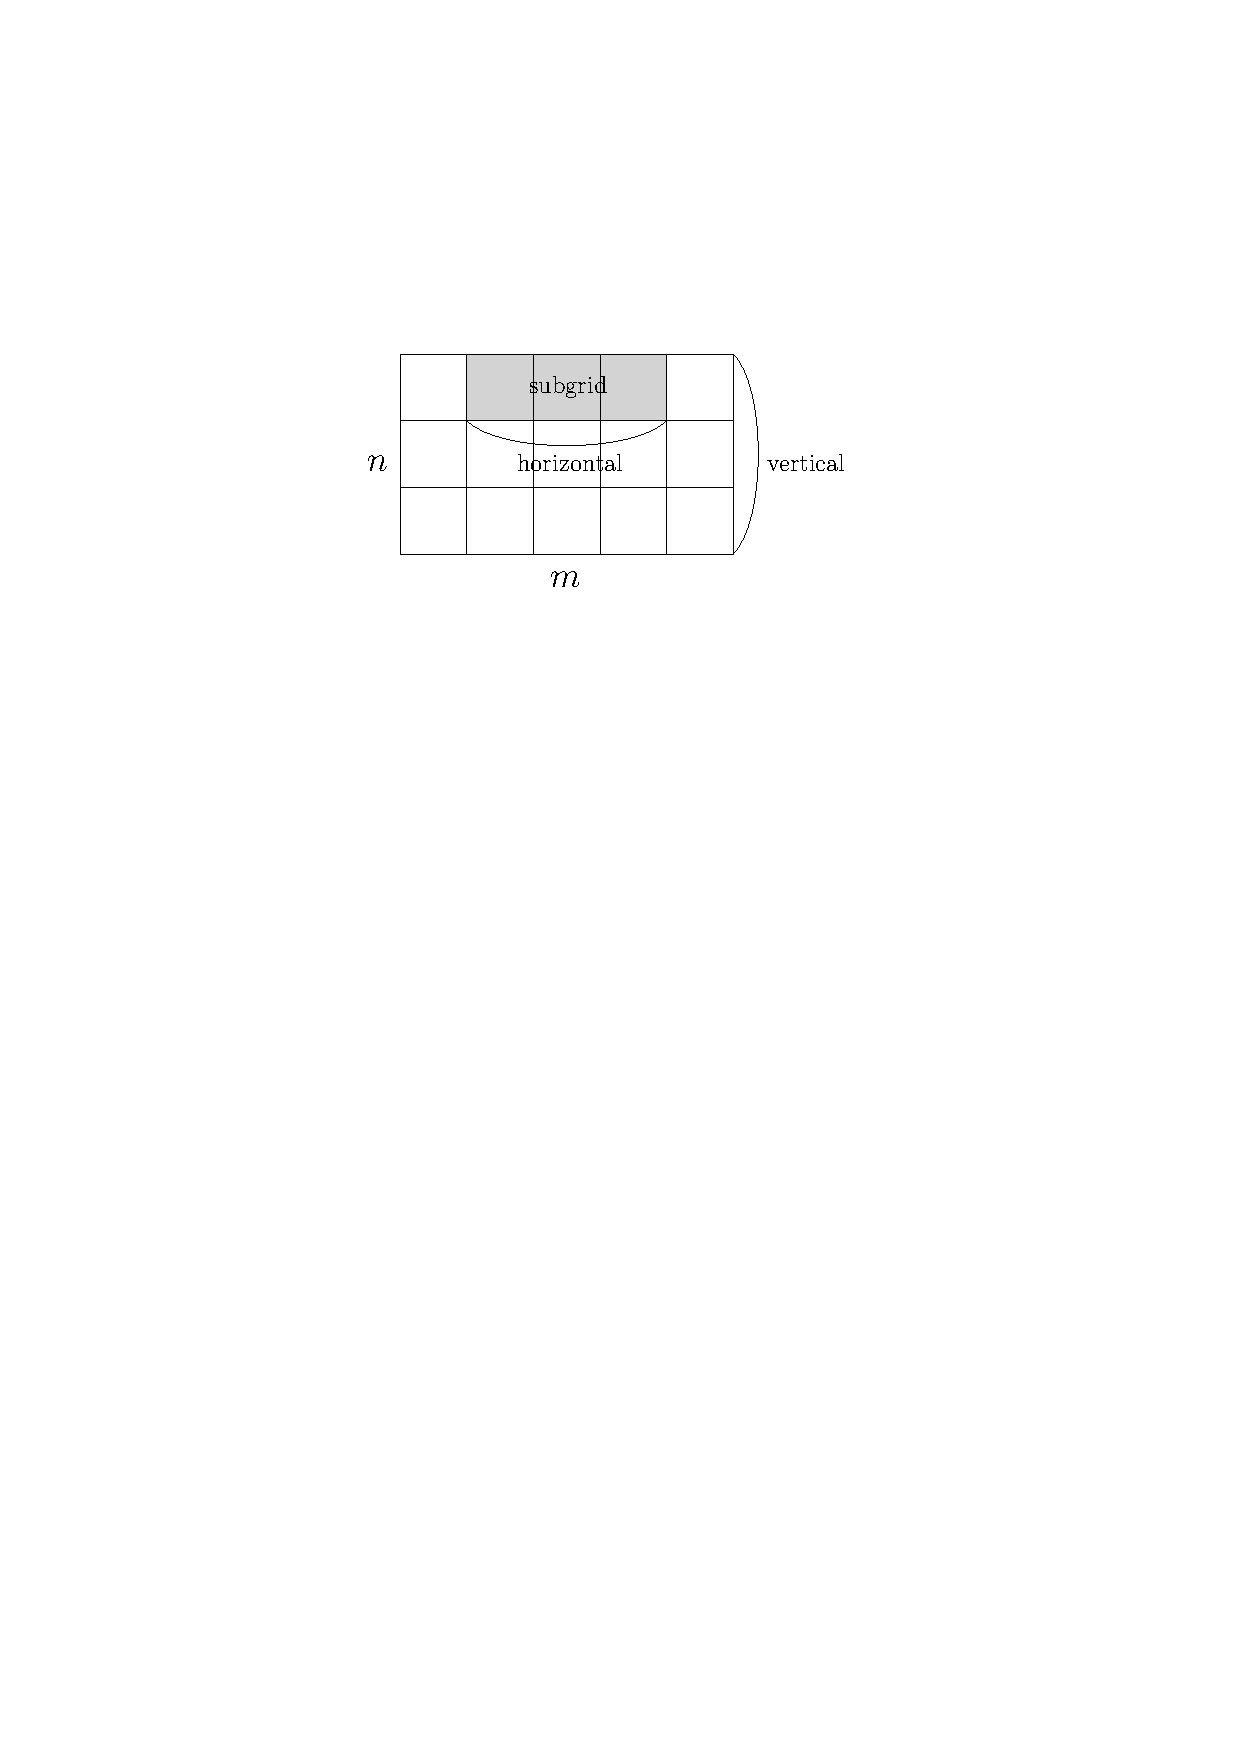
\includegraphics[scale=0.7]{examplegrid_fig.pdf}
  	\caption{In this figure only a subset of the edges of the $(m,n)$-grid appears (in this case $m=6$ and $n=4$). A $(4,2)$-subgrid of our grid is depicted in gray.} 
  	\label{fig:examplegrid}
  \end{figure}

A vertex in an oriented graph is called a \emph{sink} if all its incident edges are incoming.
An orientation of a grid is a \emph{unique sink orientation}, or \emph{USO}
for short, if all its non-empty subgrids have a unique sink. For simplicity, we call a grid with a unique sink orientation a grid USO.

Given a grid USO the task is to find the global sink. 
We assume that the orientations of the edges are given by means of a \emph{vertex oracle} which supports \emph{vertex queries} of the form: Given a vertex of the grid, reveal the orientations of the edges adjacent to this vertex.
In this paper, we study the following question: how many vertex queries suffice to find the sink of a grid USO of certain size?

%\begin{lemma}[Product construction]
% Let $G$ be an $X\times Y$-grid USO for some sets $X$ and $Y$ and let $A \subset 2^X$ and $B \subset 2^Y$ be partitions of $X$ and $Y$, respectively. Let $H$ be an $A\times B$-grid. \JN{See Malte's 4$\times$4 lower bound for a possible way to define this.}
%\end{lemma}


\subsection{Summary of results}

We assume that a unique sink orientation of an $(m,n)$-grid $G$ is given to
us by means of a \emph{vertex oracle}.
A \emph{sink-finding algorithm for the $(m,n)$-grid} is any procedure which
eventually queries the sink of $G$.
In this paper we pursue the following question:
\begin{quote}
    Among all deterministic sink-finding algorithms $\cal A$ for the
    $(m,n)$-grid, what is the minimum number of queries that $\cal A$ must ask
    in the worst case?
\end{quote}
Throughout the paper we will denote this number by $t(m,n)$.
Our results are:

\begin{itemize}
    \item
        $t(m,n) \in O(N (\log N)^2)$, where $N = m+n$. (Theorem~\ref{theorem:Sink algorithm})
    \item
        $t(m,n) \ge m+n-1$ (Theorem \ref{thm:lowerbound}), and this is optimal at least in
        the following cases:
        \begin{itemize}
            \item $m=2$ or $n=2$ (Theorem \ref{}),
            \item $(m,n) = (3,3)$ (Theorem \ref{}),
            \item $(m,n) = (4,4)$ (Theorem \ref{}).
        \end{itemize}
\end{itemize}

\section{Induced USOs}

When designing algorithms for grids, at some point one will typically want to
partition the grid into blocks.
If such a partition into blocks forms itself a grid,
then we define an induced orientation on it.
An example of such an induced unique sink orientation is shown in figure
\ref{fig:induced}.

Formally, let $G = K_X \times K_Y$ be an oriented grid,
and let $A$ and $B$ be partitions of $X$ and $Y$, respectively.
We study the grid $H = K_A \times K_B$.
For every vertex $x = (a,b)$ of $H$, let $G(x)$ (or simply $G(a,b)$)
denote the $a \times b$-subgrid of $G$ oriented as follows:
Given two adjacent vertices $x$ and $y$ of $H$, we say that $x\succeq y$ if the sink of $G(x)$ has at least one outgoing edge to a vertex of $G(y)$. We say that is orientation is \emph{induced} on $H$ by $G$.

\begin{lemma}[USO-Lemma]\label{lemma:USO-Lemma}
Let $G = K_X \times K_Y$ be an oriented grid,
and let $A$ and $B$ be partitions of $X$ and $Y$, respectively.
The orientation of the grid $H = K_A \times K_B$ induced by $G$ is a unique sink orientation.
\end{lemma}
\begin{proof}
Note that it suffices to prove that every $(2,2)$-subgrid of $H$ has a unique sink orientation. Indeed, if $H$ has at least two sinks, then any $(2,2)$-subgrid containing them has no unique sink orientation.

Let $a, a'\in A$ and $b,b'\in B$. Let $F$ be the $\{a,a'\}\times\{b, b'\}$-subgrid of~$H$.
Note that $F$ consists of four vertices being $(a,b), (a', b), (a, b')$ and $(a', b')$.
We claim that $F$ has a unique sink orientation. 
To prove this claim, we need to show that $F$ has exactly one sink.
We first show that $F$ has at most one sink.
To this end, assume for a contradiction that $F$ has more than one sink.
Since these sinks cannot be adjacent, $F$ can have at most two sinks.
Assume without loss of generality that $(a',b)$ and $(a, b')$ are the sinks of $H$.
Therefore, $(a, b)$ (and analogously $(a', b')$) has its edges oriented towards both $(a',b)$ and $(a, b')$.

Let $s_{a,b}, s_{a, b'}, s_{a'b'}$ and $s_{a', b}$ be the sinks of $G(a,b), G(a,b'), G(a',b')$ and $G(a',b)$, respectively.
By the definition of the orientation of $H$, we know that $s_{a,b}$ has at least one outgoing edge to a vertex in $G(a, b')$ and another to a vertex in $G(a', b)$. Thus $s_{a,b}$ is smaller than both $s_{a,b'}$ and $s_{a',b}$ by transitivity. Analogously, we can show that $s_{a',b'}$ is also smaller than both $s_{a,b'}$ and~$s_{a',b}$. 

Consider the $(2,2)$-subgrid of $G$ containing both $s_{a,b'}$ and~$s_{a',b}$. Note that $s_{a,b'}$ and~$s_{a',b}$ are not adjacent in this grid. Let $p$ and $q$, be the other two vertices of this grid, where $p\in G(a, b)$ while $q\in G(a', b')$; see Figure~\ref{}.
Because $p$ is smaller than $s_{a, b}$, we conclude that $p$ is also smaller than both $s_{a,b'}$ and~$s_{a',b}$. Analogously, since $q$ is smaller than $s_{a',b'}$, we know that $q$ is also smaller than $s_{a,b'}$ and~$s_{a',b}$. That is, the $(2,2)$-subgrid of $G$ containing both $s_{a,b'}$ and~$s_{a',b}$ has two sinks---a contradiction to the unique sink orientation of $G$ which comes from assuming that $F$ had at least two sinks.
Therefore $F$ has at most one sink.

To show that $F$ has a USO, we need only to prove that $F$ has no cycles.
If there is a cycle $(a,b)\succeq (a', b) \succeq (a', b') \succeq (a, b') \succeq (a,b)$, then
this induces a cycle among $s_{a,b}, s_{a, b'}, s_{a'b'}$ and $s_{a', b}$ contradicting the USO of $G$. Consequently, $F$ has a unique sink orientation.
\end{proof}

\begin{corollary}
Let $G = K_X \times K_Y$ be an oriented grid,
and let $A$ and $B$ be partitions of $X$ and $Y$, respectively.
If $(a,b)$ is the sink of the grid $H = K_A \times K_B$, then the sink of $G(a,b)$ is the sink of $G$.
\end{corollary}
\begin{proof}
Let $s_{a,b}$ be the sink of $G(a, b)$ and let $s_G$ denote the sink of $G$.
We claim that $s_G = s_{a,b}$.
Assume for a contradiction that $s_{a,b}\neq s_G$.
Note that $s_G$ does not belong to $G(a,b)$ as $s_{a,b}$ is its sink.
Therefore, $s_G$ is the sink of $G(a', b')$ for some $a'\in A, b'\in B$.

Consider the smallest subgrid in $H$ containing both $(a,b)$ and $(a', b')$. 
Since Lemma~\ref{lemma:USO-Lemma} guarantees that $(a', b')$ is not the sink of this subgrid, there is at least one outgoing edge from $(a', b')$ to another vertex. Thus, by the definition of the orientation of $H$, there is an outgoing edge going from the sink of $G(a', b')$, i.e., an outgoing edge from $s_G$---a contradiction since $s_G$ is the sink of $G$ and has no outgoing edges. Therefore, $s_G = s_{a,b}$.
\end{proof}

\section{The sink-finding algorithm}

We define a partial order of vertices in a grid unique sink orientation $G$ as follows. For any two vertices $v,w \in G$ consider the smallest subgrid containing both $v$ and $w$. We say that $w \succeq v$ if there is a path from $w$ to $v$ in this subgrid. As the grid USO is acyclic, this defines a partial order on the vertices. Note that the sink of the grid is the unique minimal vertex with respect to this ordering. 

Note that two vertices may not be $\succeq$-comparable in the smallest subgrid containing them. Thus\JN{after the transitive closure they might still be incomparable}, we consider the transitive closure of this relation and say that a vertex $w$ is \emph{larger} than $v$ (or $v$ is smaller than $w$) if there is a sequence $w = v_1, v_2, \ldots, v_k = v$ of $G$ such that $v_i \succeq v_{i+1}$, for each $1\leq i\leq k-1$.

In a grid USO $G$, the \emph{\indegree} of a vertex $v \in G$ is an ordered pair $[a_v, b_v] \in \{0,1,\ldots,|X|-1\}\times \{0,1,\ldots,|Y|-1\}$ where $a_v$ and $b_v$ specify the number of incoming horizontal  and vertical edges of $v$, respectively.

\begin{lemma}
 Given an $(n, n)$-grid USO we can find a vertex with a \indegree $[a,b]$ satisfying $a, b \geq \frac{n}{4} - 1$ by using $\mathcal{O}(n)$ vertex queries.
\end{lemma}

\begin{proof}
The algorithm we describe queries a linear number of vertices of the grid before finding a vertex with the required \indegree. 
After explaining the algorithm we prove its correctness.
  
The algorithm works as follows. First, query the diagonal vertices $D = \{v_1,\ldots, v_n\}$ where $v_i = (i,i)$. If one of the vertices in $D$ has the required \indegree, we are done. If not, assume without loss of generality that $v_i \succeq v_j$ whenever $j > i$; otherwise rename the vertices. 
With this assumption, we claim that every diagonal vertex $v_i \in D$ has at least $i - 1$ incoming edges. Indeed, for each $j < i$, we have that either $v_j \succeq v_i$ or they are incomparable. Thus, regardless of the case we can guarantee the existence of at least one incoming edge to $v_i$ in the $(2, 2)$-subgrid containing $v_i$ and $v_j$. 

Let $V = \{v_{\lceil n/2 \rceil},\ldots,v_n\} \subseteq D$.
Label the vertices in $V$ as \emph{horizontal}  or \emph{vertical}, if the majority of incoming edges for the corresponding vertex are horizontal  or vertical, respectively. 
Assume without loss of generality that there are more vertical vertices in $V$; otherwise change the role of the coordinates. 
Let $V' \subseteq V$ be the set of all vertical vertices in $V$ and notice that $|V'| \geq |V|/2$.
 Additionally, let $v$ be a minimal vertex of $V'$, i.e., for each $u\in V'$ either $u\succeq v$, or $u$ and $v$ are incomparable. 

Let $I'$ be the set of indices containing the first coordinate of each vertex in~$V'$.
Assume that $v = (x_v, y_v)$ and let $W = I'\times \{y_v\}$ be the set of vertices in the same row as $v$ and in the same column as some other vertex from $V'$.
To conclude, the algorithm queries each vertex in $W$.
It is clear from the description above that the number of vertices queried so far is $|D| + |W| = \mathcal{O}(n)$. 
We claim that one of the queried vertices will have the required \indegree.

To prove our claim, recall that every diagonal vertex $v_i \in D$ has at least $i - 1$ incoming edges.  
Therefore, each vertex of $V'$ has at least $\lceil n/2 \rceil - 1$ incoming edges. 
Moreover, each vertex in $V'$ has at least $\frac{\lceil n/2\rceil-1}{2}$ incoming vertical edges and $|V'| \geq \frac{n-\lceil n/2\rceil + 1}{2} \geq \frac{n}{4}$. 

Let $v^*$ be the sink of $W$ obtained after querying each vertex in this set (including $v$). Let $[a,b]$ be the \indegree of $v^*$. We claim that $a, b \geq \frac{n}{4} - 1$. 
Indeed, because $v^*$ is smaller than each other vertex in $W$, we know that $$a \geq |W|-1 = |V'|-1 = \frac{n-\lceil n/2\rceil + 1}{2} - 1 \geq \frac{n}{4} - 1.$$


If $v = v^*$, then since $v\in V'$, we know that $b\geq \frac{\lceil n/2\rceil-1}{2}\geq \frac{n}{4} - 1$.
Otherwise, there is a vertex $w \in V'$ that is in the same column as $v^*$.
  This situation is depicted in Figure~\ref{fig:seedlem1}.
  \begin{figure}[htbp] 
  	\centering
  	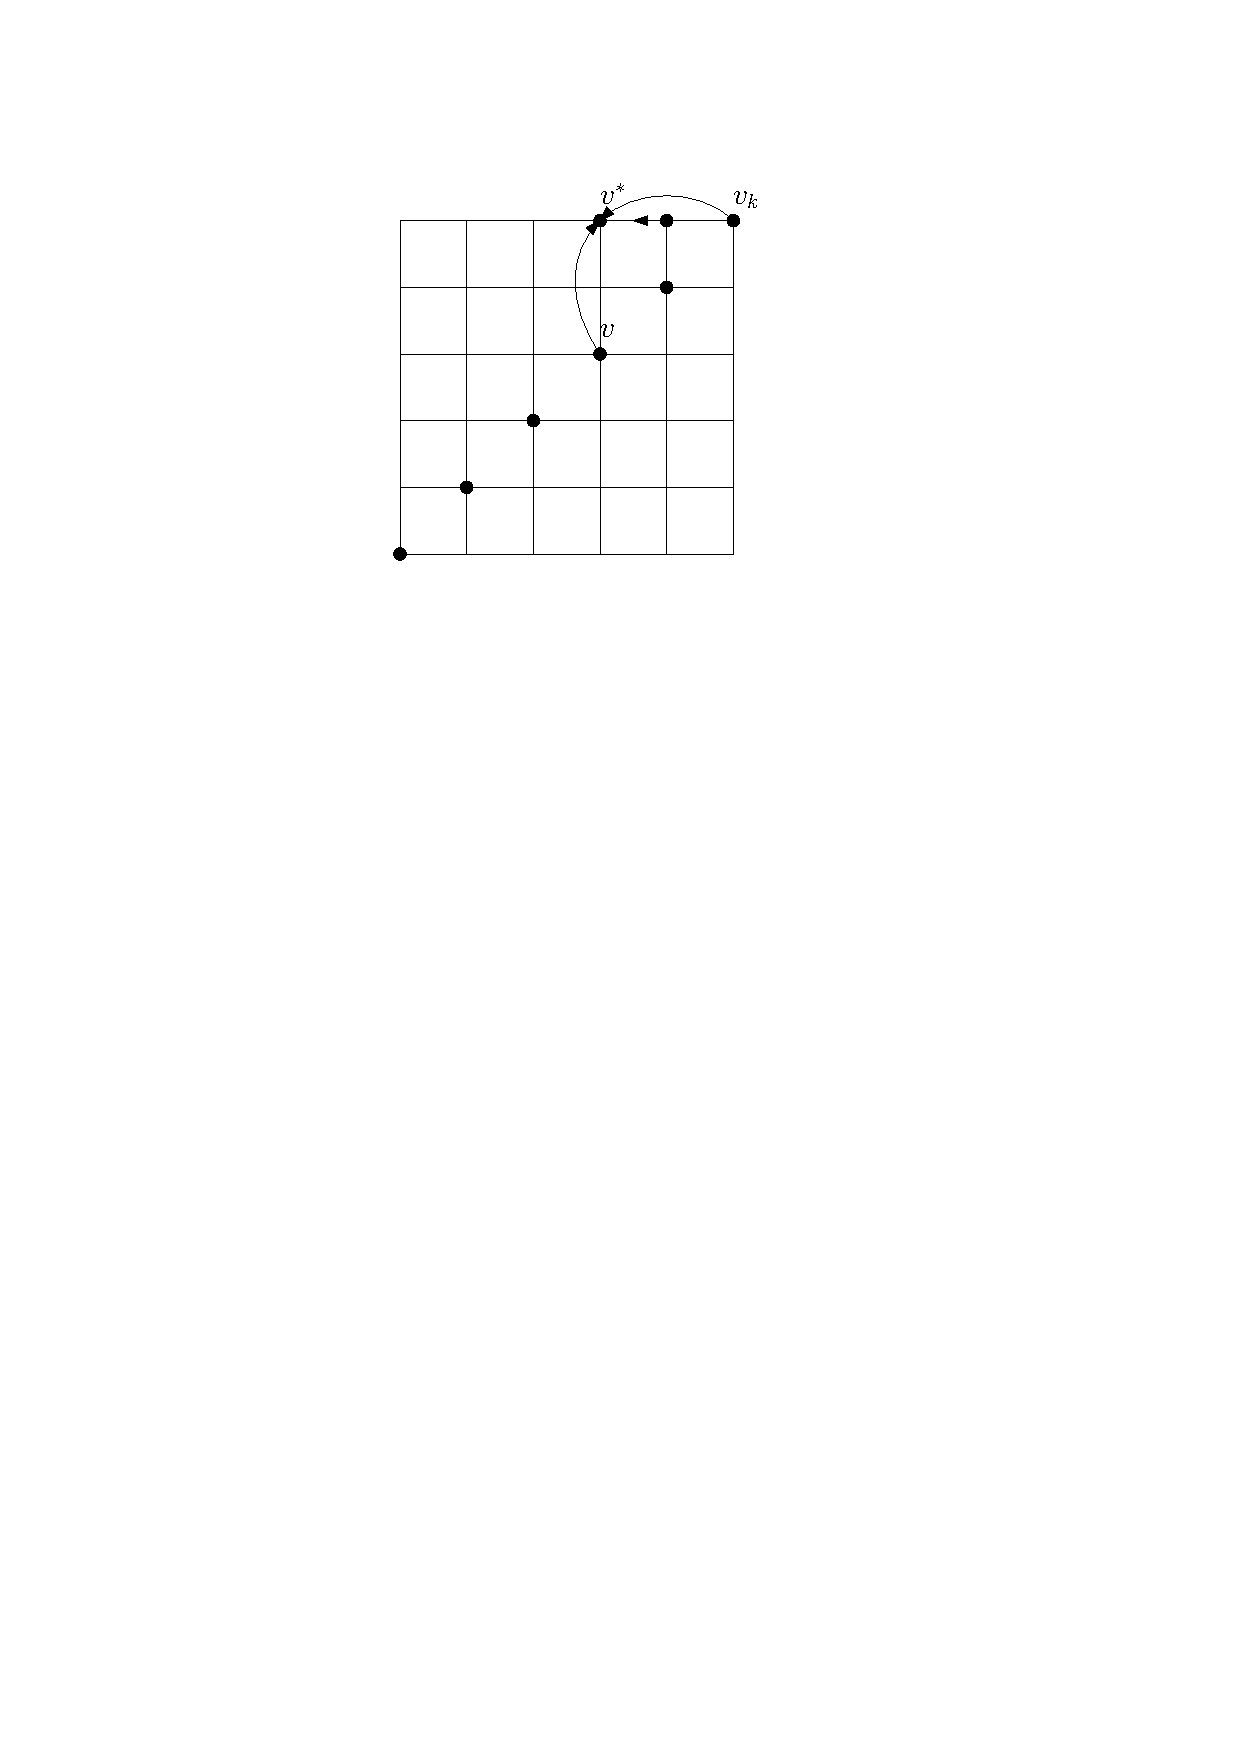
\includegraphics[scale=0.7]{seedlemma_fig1.pdf}
  	\caption{In this figure only a subset of the edges of the grid appears. The vertices that are marked with discs are the ones evaluated.} 
  	\label{fig:seedlem1}
  \end{figure}
   If we can show that there is an edge from $w$ to $v^*$, then by acyclicity $v^*$ has at least one more incoming vertical edge as compared to $w$, therefore establishing that $b \geq \frac{\lceil n/2\rceil-1}{2} + 1 \geq \frac{n}{4} \geq \frac{n}{4} - 1$. 
   
   Because $v$ is a minimal vertex in $V'$, either $w\succeq v$, or $v$ and $w$ are incomparable. 
   To show that there is an edge from $w$ to $v^*$ we study these two cases: 
   
If $w \succeq v$, then because $v \succeq v^*$ we have due to transitivity that $w \succeq v^*$. 
  Otherwise, $w$ and $v$ are incomparable. In this case, since $v^*$ is smaller than $v$, we know that the edge connecting $v$ and $v^*$ is  oriented towards $v^*$. Therefore, the only possibility for $v$ and $w$ to be incomparable is that there is an edge from $w$ to $v^*$. We give illustrations of the two cases in Figure~\ref{fig:seedlem2}. Thus regardless of the case, there is an edge from $w$ to $v^*$ which concludes the proof.   
   \begin{figure}[htbp] 
       \centering
       \begin{subfigure}[b]{0.4\textwidth}
           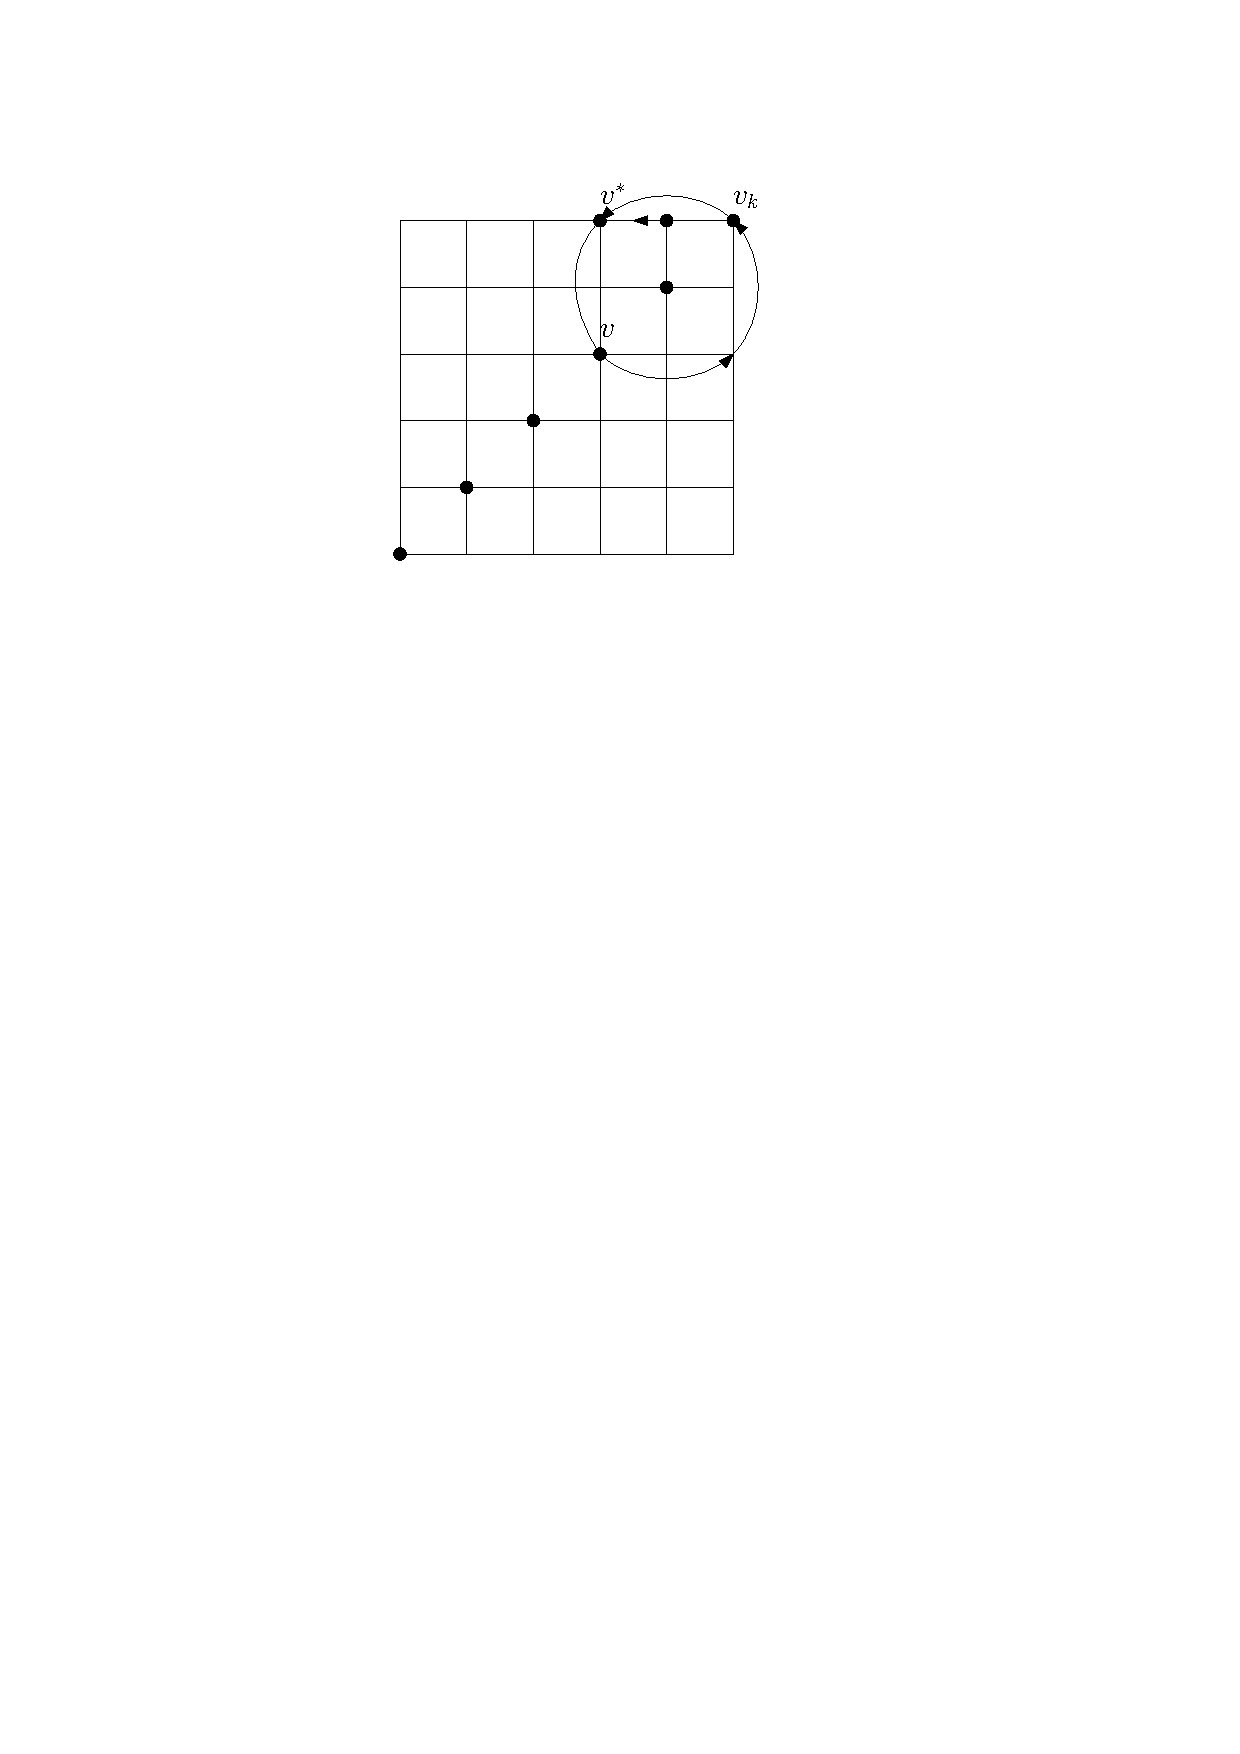
\includegraphics[scale = 0.7]{seedlemma_fig2_cas1.pdf}
           \caption{$w \succeq v$}
       \end{subfigure}
       \qquad \qquad
       \begin{subfigure}[b]{0.4\textwidth}
           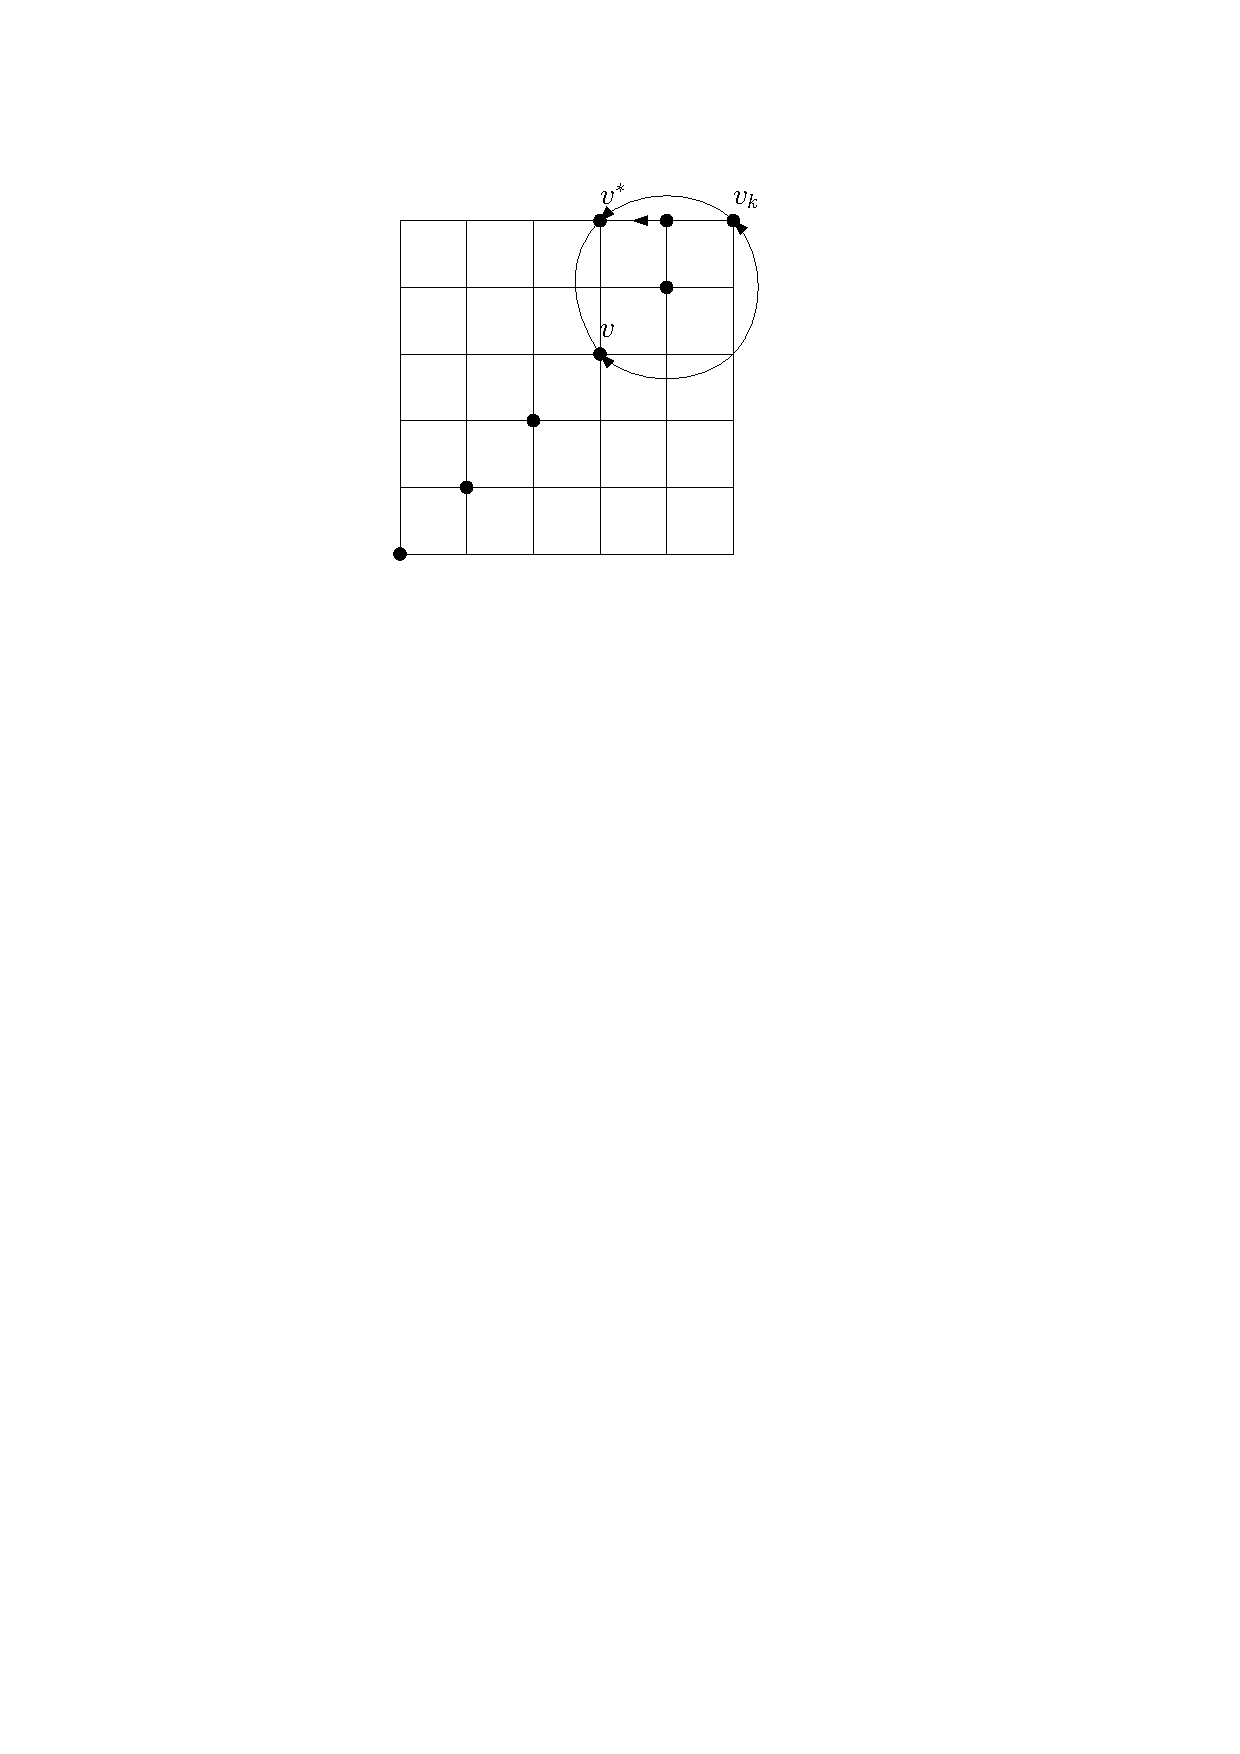
\includegraphics[scale = 0.7]{seedlemma_fig2_cas2.pdf}
           \caption{$v$ and $w$ are incomparable}
       \end{subfigure}
       \caption{Illustrations of the two cases. }
       \label{fig:seedlem2}
   \end{figure}
\end{proof}

\begin{corollary}\label{corollary: n/4 indegree}
 Let $M = \max\{m,n\}$. Given a grid $K_{m} \times K_{n}$, we can find a vertex with \indegree $[a,b]$ with $a \geq \frac{m}{4} - 1$ and  $b \geq \frac{n}{4} - 1$ using $\mathcal{O}(M)$ vertex queries.
\end{corollary}

\begin{proof}
 Use the product construction and divide the columns into blocks of size $\frac{m}{n}$.
 %Without loss of generality assume that $m \geq n$. Assume also for the ease of description that $n$ divides $m$. We will deal with this assumption in the end. Divide the columns into $n$ blocks of size $\frac{m}{n}$. More specifically, partition $[m]$ into $n$ parts $I_1, \ldots, I_n \subseteq [m]$ with $|I_j| = \frac{m}{n}$ for all $j = 1,\ldots, n$. 
 %We are going to consider the subgrids of the form $K_{I_j}\times K_{\{j\}}$. Notice that each subgrid is a fraction of a different row and consists of $\frac{m}{n}$ vertices. We query all the vertices in these subgrids for a total of $m$ vertex queries therefore finding also the sink $s_j$ in each subgrid $K_{I_j}\times K_{\{j\}}$. Consider any linear extension of the partial order induced by the relation $\succeq$ on the set $\{s_1, \ldots, s_n\}$. We can assume that the order of the indices coincides with the linear extension, otherwise just rename them. Notice that $s_j$ has at least $j\cdot\frac{m}{n} - 1$ incoming edges (to see that, compare $s_j$ with all the vertices in the subgrids whose sinks are $s_1,\ldots,s_{j-1}$ and the subgrid containing $s_j$). Consider the set $S = \{s_{ n/2 },\ldots, s_n\}$ \JN{We need to somehow deal with parity of $n$.}. Assume that for at least half of the $s_j$'s the majority of the incoming edges are vertical (the horizontal case is similar and easier) and let $S' \subseteq S$ be the set of such $S_j$'s. That is, every $s_j \in S'$ has at least $\frac{1}{2}\left(j\cdot\frac{m}{n} - 1\right)$ vertical incoming edges. Now $|S'| \geq \frac{n}{4}$ and every vertex has at least $\frac{1}{2}\left(\frac{n}{2}\cdot\frac{m}{n} - 1\right) = \frac{m}{4}-\frac{1}{2}$ many incoming vertical edges.
\end{proof}



%if every induced directed subgraph that is attained by fixing or limiting the range of some coordinates of the vertices has a unique sink. More specifically, we require this property to hold for subgraphs that are attained by taking $d$ nonempty index sets $\emptyset \not= J_i \subseteq \mathbb{Z}_n, i = 1,\ldots,d$ and considering the induced subgraph over the vertices $\{(a_1,\ldots, a_d) \in V \: : \:  a_i \in J_i \: \forall i = 1,\ldots, d \}$. If each $J_i$ is the whole of $\mathbb{Z}_n$ or a singleton, we call the resulting induced subgraph a \emph{face}. The dimension $d' \in \{0,1,\ldots, d\}$ of the face is the number of index sets that are the whole of $\mathbb{Z}_n$. Note that a face of $(K_n)^d$ of dimension $d'$ is isomorphic to $(K_n)^{d'}$. Any face can be compactly written as a vector $(v_1,\ldots,v_d) \in \left(\mathbb{Z}_{n} \cup \{*\}\right)^d$ where $v_i$ matches the only element of $J_i$ when $J_i$ is a singleton and $v_i$ is $*$ otherwise. Unless otherwise clear, one should also specify what $n$ is when talking of faces. This concept of a face is a natural generalization from the $d$-cube $(K_2)^d$ for which the faces we defined correspond to the faces of the $d$-cube in the geometric sense.

%Consider some USO of $(K_n)^d$. For this USO we define the \emph{in-map} $\phi : V \rightarrow \mathbb{Z}_n^d$ for each vertex $v = (v_1,\dots, v_d) \in V$ so that $\phi(v)_i$ is the number of edges that are incoming for $v$ from its neighbors $w \in V$ that differ from $v$ on coordinate $i$. It was shown by \citet[Theorem 2]{gartner2008unique} that for a USO this mapping is infact a bijection. The \emph{product construction} for grids (\citet{gartner2008unique}, \citet{szabo2001unique}) states that we can contract dimensions and maintain the USO structure. More specifically, for any $I \subseteq \mathbb{Z}_n$ consider the set of faces 
% \begin{align*}
%  G = \{(a_1,\ldots,a_n) : a_i = * \textnormal{ if } i \in I \textnormal{ and } a_i \in \mathbb{Z}_n \textnormal{ otherwise}\}.
% \end{align*}
% Note that $|G| = n^{d-|I|}$ and there is a natrual way to consider a USO over a graph whose vertices are the faces in $G$: for any $f \in G$ its neighbors are those faces that differ from it in the fixed coordinates and the orientation of the edges is determined by the orientation of the corresponding edges in the sink of $f$. This definition turns out to be well defined and the arising structure forms a USO that is over a graph isomorphic to $(K_n)^{d-|I|}$. 
% 
% 
% The problem we are looking at is that of finding the global sink of a USO over $(K_n)^d$. The USO is given by an oracle that for any given vertex reveals the orientations of the edges adjacent to the vertex. The question is, what is the least number of these vertex queries needed to find the unique global sink? Just knowing its location is not sufficient, but we also require that the sink is evaluated. This requirement will prove useful when developing an algorithm.


\subsection{Hitting the wall}

Given a vertex $v = (x_v, y_v)$ with \indegree $[a, b]$ in a grid USO $G$, let $I_v\subseteq [m]$ be the set of indices such that  $I_v \times \{y_v\}$ is the set of all vertices with an outgoing horizontal edge to $v$ with $v$ included in this set. Analogously, $J_v\subseteq [n]$ is the set of indices such that $\{x_v\}\times J_v$ is the set of all vertices with an outgoing vertical edge to~$v$ (including $v$). Notice that $|I_v| = a + 1$ while $|J_v| = b + 1$.

\begin{lemma}\label{lemma:Sink of dominated grid}
Given a vertex  $v = (x_v, y_v)$ in a grid USO $G$, $v$ is the sink of the $I_v\times J_v$-grid.
\end{lemma}
\begin{proof}
Vertex $v$ has only incoming edges in the $I_v\times J_v$-grid and is therefore the unique sink of this subgrid of $G$. 
%Assume for a contradiction that there is a vertex $z = (x_z, y_z)$ of the $I_v\times J_v$-grid such that $z$ is smaller than $v$. Let $u = (x_z, y_v)$ and $w = (x_v, y_z)$ the other two vertices of the $\{x_v, x_z\}\times\{y_v,y_z\}$-grid.
%Since $x_v\in I_v$ and $y_v\in J_v$ and by the definition of $I_v$ and $J_v$, we know that $v$ is smaller than both $u$ and~$w$.
%Because we assumed that $z$ is smaller than $v$, by transitivity we know that both $u$ and $w$ are also smaller than $z$. Therefore, both $z$ and $v$ are sinks of the $\{x_v, x_z\}\times\{y_v,y_z\}$-grid---a contradiction to the USO property that comes from assuming that $z$ is smaller than $v$. Therefore, $v$ is the sink of the $I_v\times J_v$-grid.
\end{proof}

In the settings of the previous lemma, we say that the $I_v\times J_v$-grid is \emph{dominated} by $v$ in~$G$.

\begin{lemma}
Given an $[m]\times[n]$-grid USO $G$ and sets $I, I'\subset [m]$ and $J,J'\subset [n]$ such that $I\cap I' = \emptyset = J\cap J'$. If $u$ is the sink of the $I\times J$-subgrid while $v$ is the sink of the $I'\times J'$-subgrid such that $v$ is smaller than $u$, then $v$ is either smaller than the sink of the $I\times J'$-grid or smaller than the sink of the $I'\times J$-grid (maybe smaller than both).
\end{lemma}


\subsection{Finding the sink}
The idea of our algorithm is the following: Using Lemma~\ref{corollary: n/4 indegree}, we find a vertex which dominates already a subgrid with at least $n^2/16$ of the vertices  by Lemma~\ref{lemma:Sink of dominated grid}. However, this is not enough so we use Lemma~\ref{lemma:Constant fraction improvement} below to find a smaller vertex that dominates a ``larger'' subgrid. By repeating this process a logarithmic number of times, we end up with a vertex whose dominated subgrid spans a strip of the original grid containing at least one eight of the vertices. This leaves us with another (non-square) grid where we can repeat our algorithm recureively. The key result to this process is described in the next lemma.


\begin{lemma}\label{lemma:Constant fraction improvement}
Let $G$ be an $[m]\times[n]$-grid USO. 
Given a vertex $v$ with \indegree $[\alpha m, \beta n]$ such that $0 < \alpha, \beta < 1$, we can compute another vertex with \indegree $[a,b]$ where either $a\geq \frac{1+7\alpha}{8}m$ and $b \geq \beta n$, or $a \geq \alpha m$ and $b \geq \frac{1 + 7\beta}{8}n$. This process requires $O(M)$ vertex queries, where $M = \max\{m,n\}$.
\end{lemma}

\begin{proof}
Assume that $(1-\alpha) m \geq (1-\beta)n$, the other case is analogous. 
Let $\rho = \lfloor \frac{(1-\alpha)m}{(1-\beta)n} \rfloor$.
We consider $\rho$ square grids defined as follows. 

Consider the  $I_v\times J_v$-subgrid dominated by $v$ and 
notice that $|I_v| = \alpha m + 1$ while $|J_v| = \beta n + 1$.

Let $\overline{I_v} = [m]\setminus I_v$ and $\overline{J_v} = [n]\setminus J_v$.
Let $A_1, \ldots, A_\rho$ be a partition of $\overline{I_v}$ into $\rho$ pairwise disjoint subsets of indices such that each has size $k = (1-\beta)n$, except maybe for the last one which contains at most $2k-1$ indices.
For each $1\leq i\leq \rho$, let $G_i$ be the $A_i\times \overline{J_v}$-grid. That is, we define $\rho$ pairwise-disjoint $(k, k)$-subgrids of $G$; see Figure~\ref{fig:Expansion Lemma 1}.

\begin{figure}[tb]
\centering
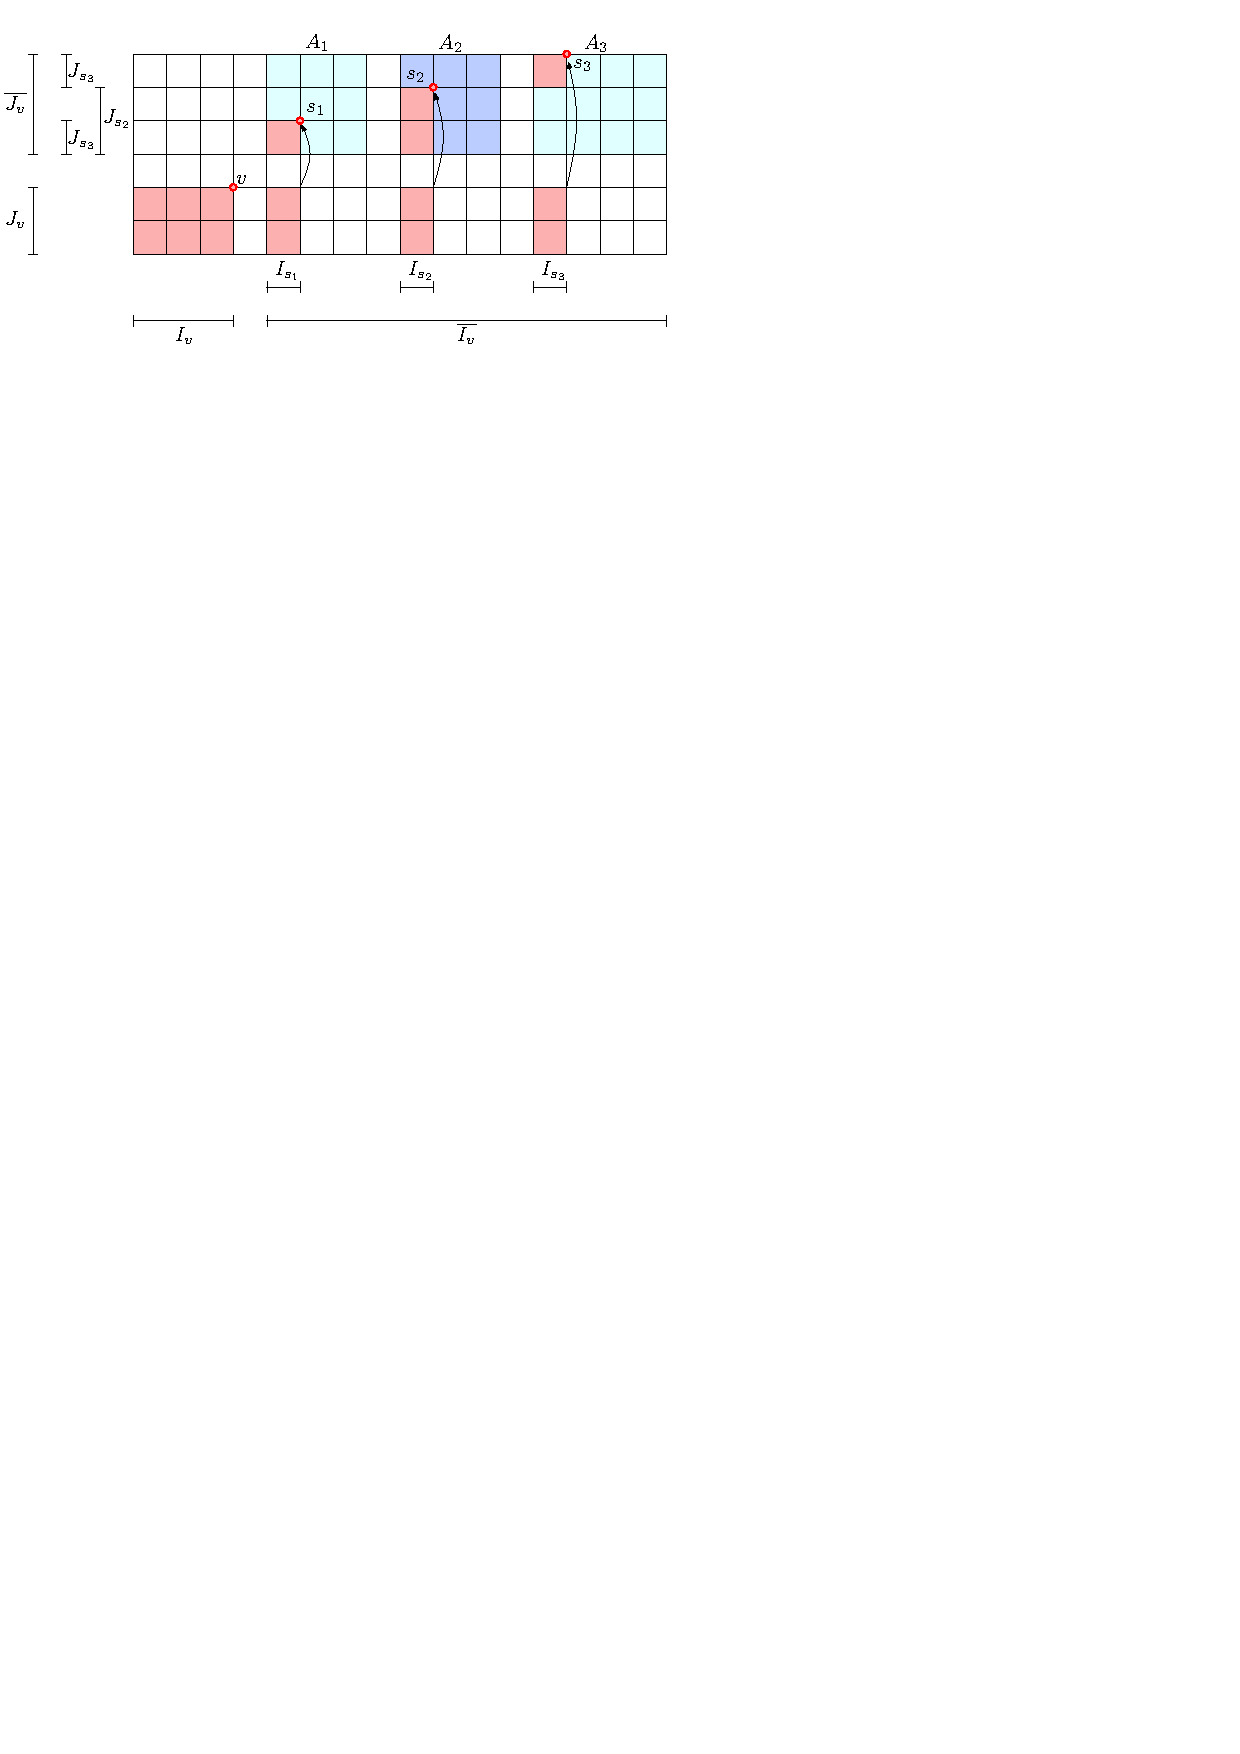
\includegraphics{expansion_lemma_fig1.pdf}
%[width=1\textwidth]
\caption{\small }
\label{fig:Expansion Lemma 1}
\end{figure}

For each $G_i$, use Corollary~\ref{corollary: n/4 indegree} to compute a vertex $s_i$ having \indegree at least $[a,b]$ in $G_i$, where $a,b \geq k/4 - 1$ (the \indegree of $s_i$ in $G$ may be larger).
By Corollary~\ref{corollary: n/4 indegree}, this requires $O(k)$ vertex queries. Since we have $\rho$ grids, with $O(k\rho) = O(m)$ vertex queries we can compute each of $s_1, \ldots, s_\rho$.
 

Consider the $I_{s_i}\times J_{s_i}$-subgrid dominated by $s_i$ in $G_i$, where $|I_{s_i}|, |J_{s_i}| \geq k/4$ and $I_{s_i}\subseteq A_i$ while $J_{s_i}\subseteq \overline{J_v}$. 
Given any $i\neq j$, notice that the set $J_{s_i}$ and $J_{s_j}$ are not necessarily disjoint whereas $I_{s_i}\cap I_{s_j} = \emptyset$; see Figure~\ref{fig:Expansion Lemma 1}.

By Lemma~\ref{lemma:USO-Lemma}, we know that $s_i$ is smaller than each vertex in either the $I_v\times J_{s_i}$-grid or the $I_{s_i}\times J_v$-grid. This yields two cases:

\textbf{Case 1:} If there exists $1\leq i \leq \rho$ such that
$s_i$ is smaller than each vertex in the $I_v\times J_{s_i}$-grid, then let $W =  \{x_{s_i}\} \times (J_v\cup J_{s_i})$ be a set of at least $\beta n + k/4$ vertices, where $s_i = (x_{s_i}, y_{s_i})$; see Figure~\ref{fig:Expansion Case 1}. 

\begin{figure}[h]
\centering
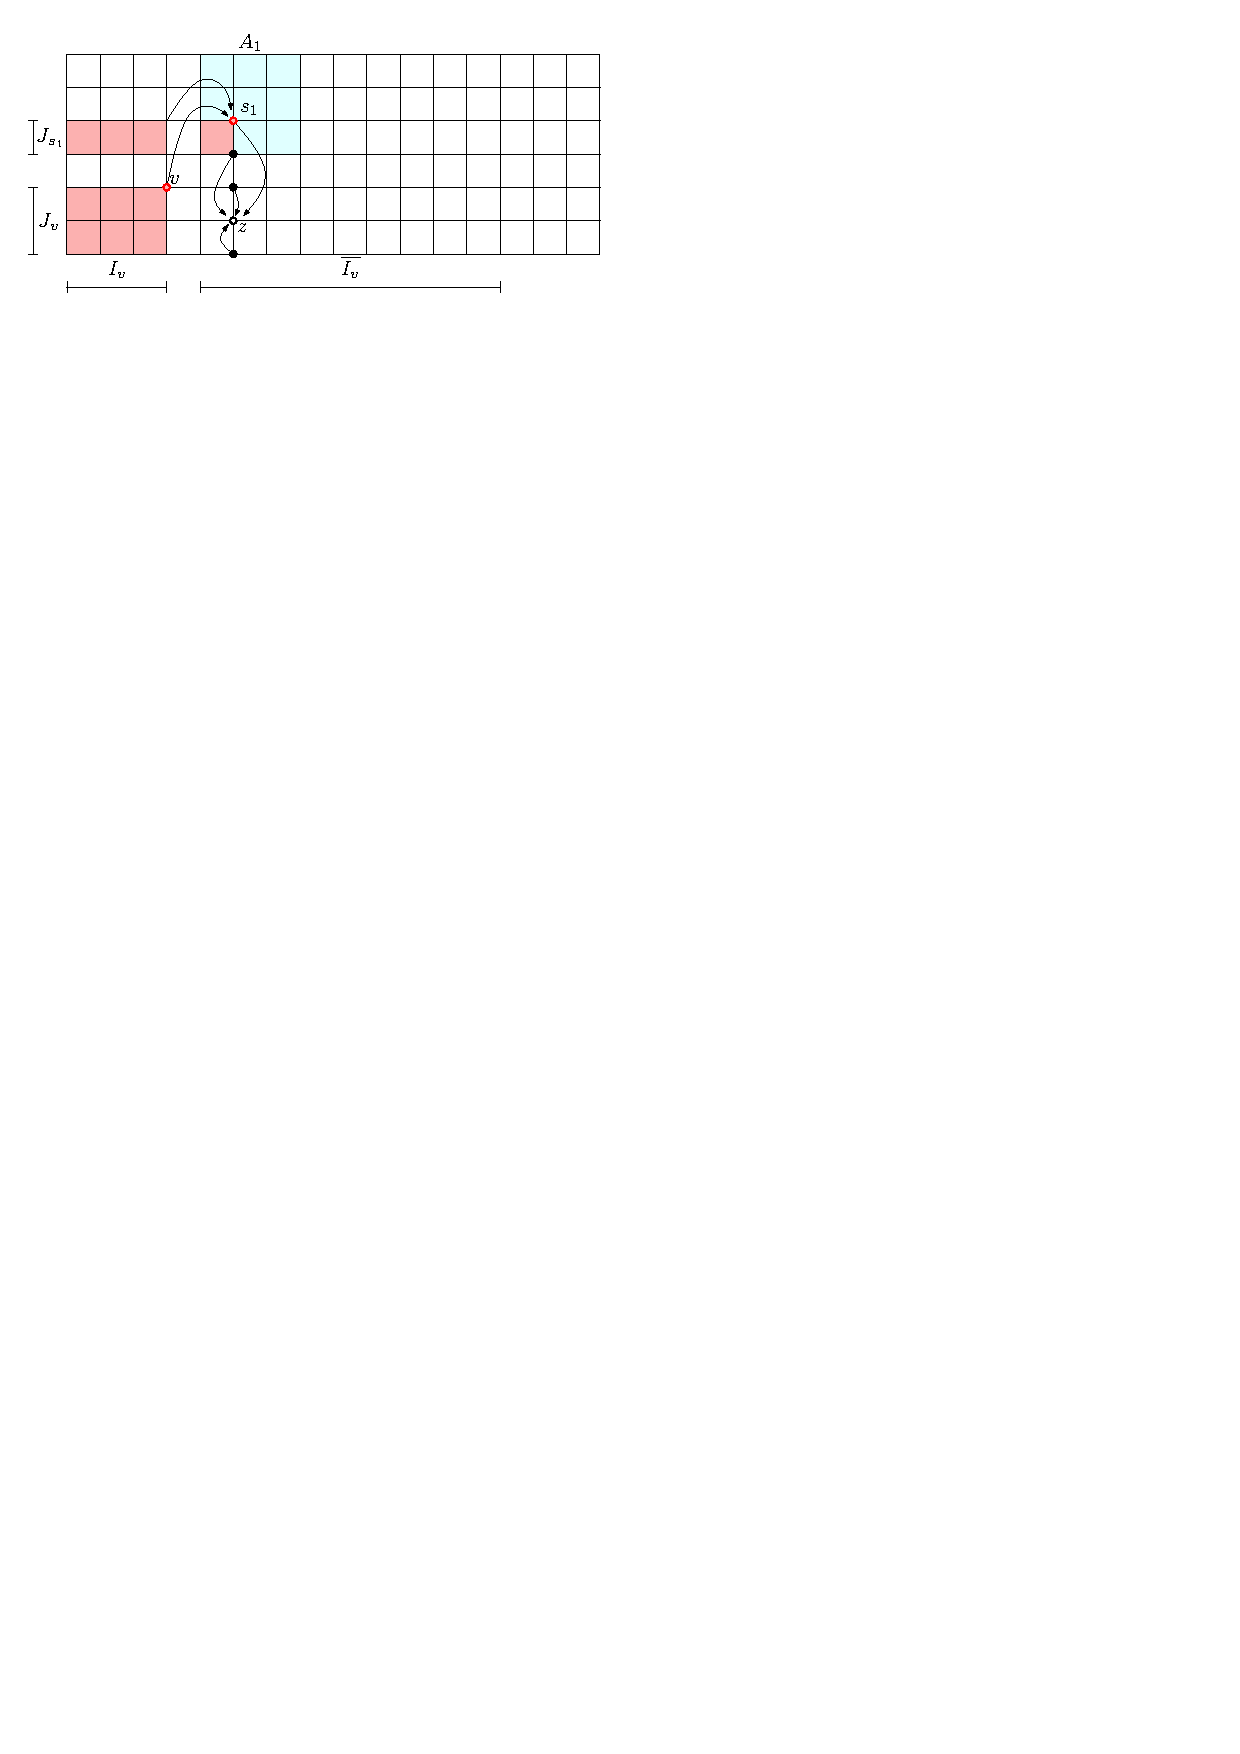
\includegraphics{expansion_lemma_Case1.pdf}
%[width=1\textwidth]
\caption{\small }
\label{fig:Expansion Case 1}
\end{figure}

Let $z$ be the sink of $W$. Note that we can compute $z$ after querying each vertex of $W$, i.e., after $O(n)$ vertex queries. Assume that $z$ has \indegree $[a_z, b_z]$. 
Because $z$ is smaller than $s_i$, $z$ is also smaller than every vertex in the $I_v\times J_{s_i}$-grid. Moreover, since $s_i$ is smaller than $v$, we know that $z$ is also smaller than $v$ and hence, $z$ is smaller than every vertex in the $I_v\times J_v$-grid.
Consequently, $z$ is smaller than every vertex in the $I_v\times (J_v\cup J_{s_i})$-grid, i.e., $a_z\geq |I_v| \geq \alpha m$.
Because $z$ is the sink of $W$, we know that
 $$b_z \geq |W| = \beta n + k/4 = \beta n + \frac{(1-\beta)}{4}n = \frac{1 + 3\beta}{4}n\geq \frac{1 + 7\beta}{8}n.$$


\textbf{Case 2:} If for each $1\leq i\leq \rho$ $s_i$ is smaller than each vertex in the $I_{s_i}\times J_v$-grid, then we want to compute a vertex that is smaller than each vertex in $S = \{s_1, \ldots, s_\rho\}$.
To this end, let $t_1 = s_1$.
For each $2\leq i\leq \rho$, let $t_{i+1}$ be the sink of the smallest subgrid containing $t_i$ and $s_{i+1}$. Note that we can compute $t_{i+1}$ with a constant number of vertex queries.
Thus, after $O(\rho)$ vertex queries, we obtain a vertex $t = t_\rho$, such that $t$ is smaller than $s_i$, for each $1\leq i\leq \rho$. Notice that $t$ lies in the same row as some $s_j\in S$ and in the same column as some $s_h\in S$, for some $1\leq j,h\leq \rho$; see Figure~\ref{fig:Expansion Case 2}. 

\begin{figure}[h]
\centering
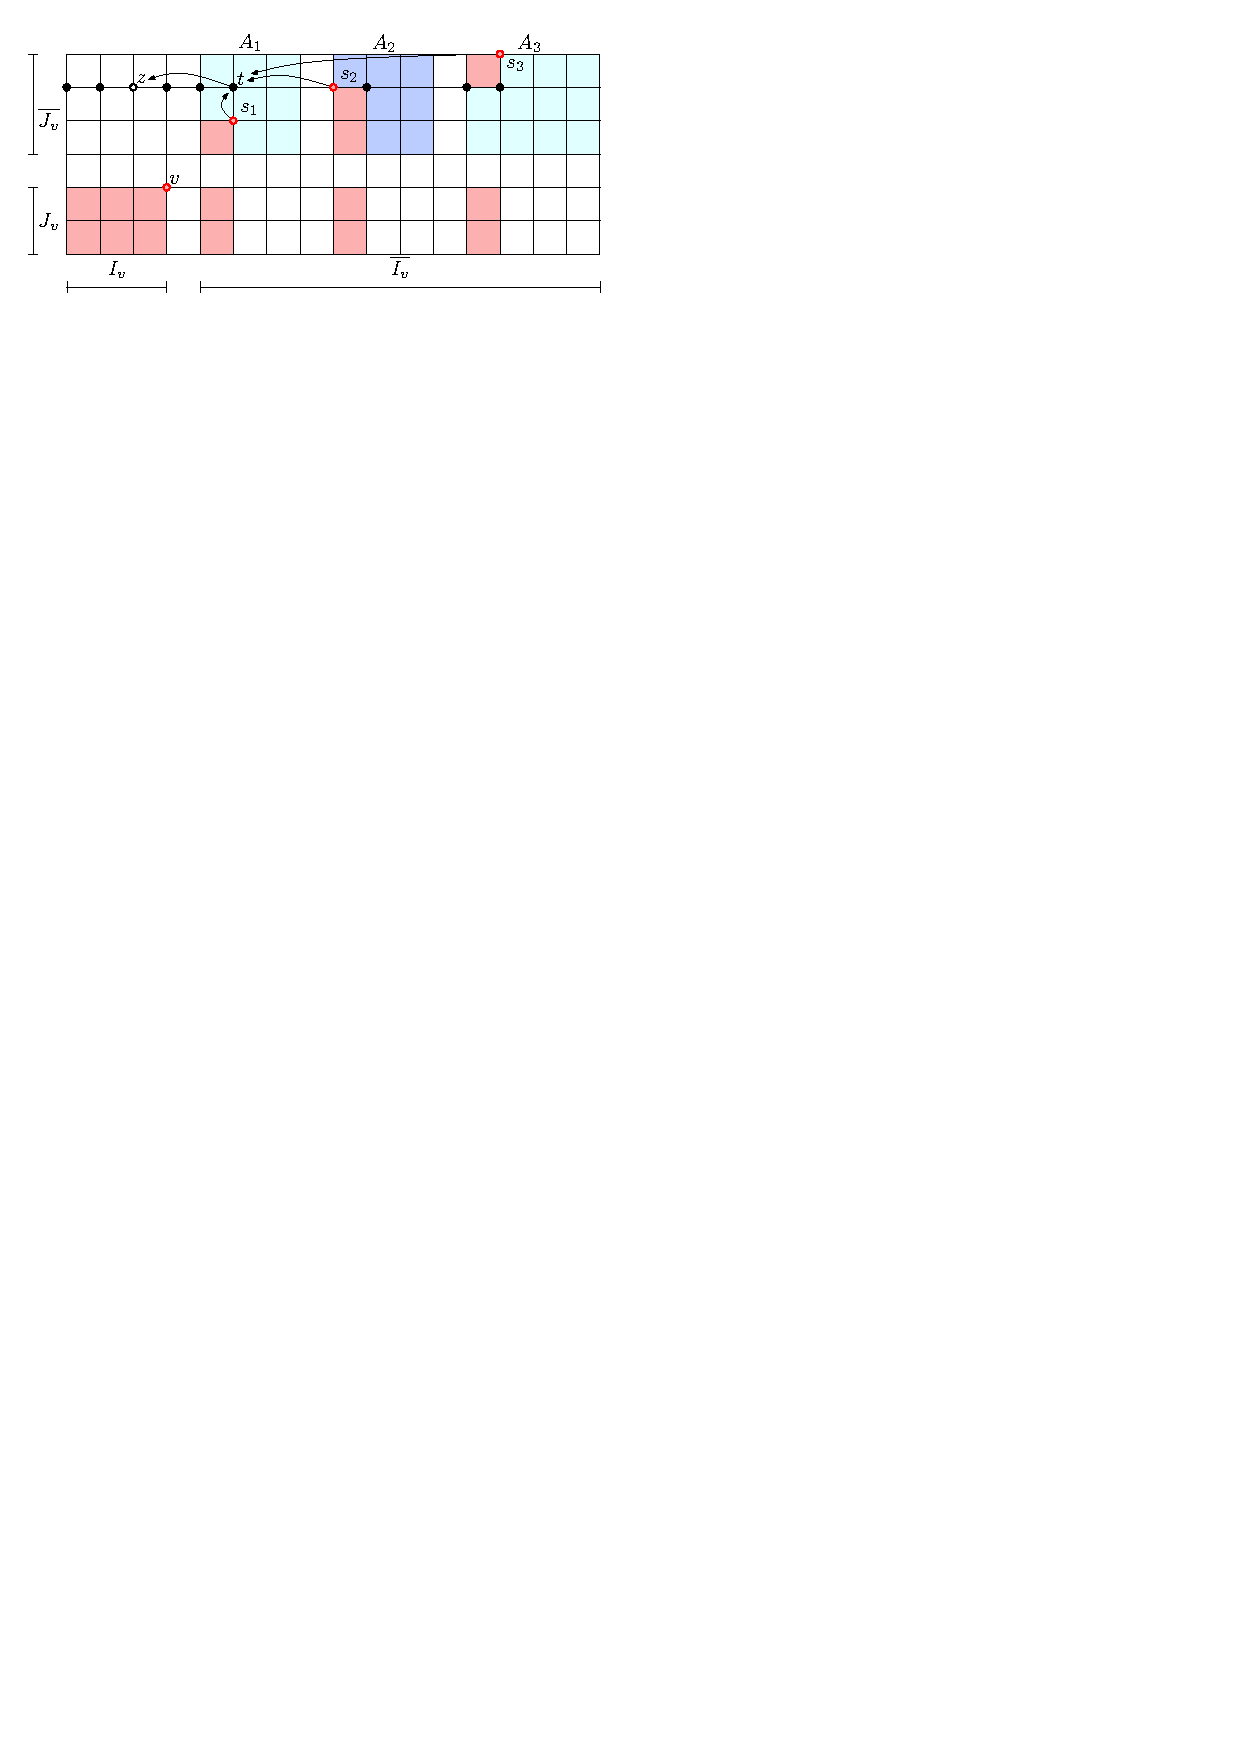
\includegraphics{expansion_lemma_fig2.pdf}
%[width=1\textwidth]
\caption{\small }
\label{fig:Expansion Case 2}
\end{figure}

Consider the following set $$W = \left(I_v\cup \left(\bigcup_{i=1}^\rho I_{s_i}\right)\right)\times \{y_t\},$$
where $t = (x_t, y_t)$.
Let $z$ be the sink of $W$ and let $(a_z, b_z)$ denote the \indegree of $z$.

Because $z$ is the sink of $W$, we infer that 
$$a_z \geq |W|  = |I_v| + \sum_{i=1}^\rho |I_{s_i}| \geq
\alpha m + \rho k/4  = \alpha m +  \left\lfloor \frac{(1-\alpha)m}{(1-\beta)n} \right\rfloor \frac{(1-\beta) n}{4}.$$

Since we assumed that $(1 - \alpha) m > (1-\beta) n$, and by the properties of the floor function, we know that $$(1 - \alpha) m \geq \left \lfloor \frac{(1-\alpha)m}{(1-\beta)n} \right \rfloor (1-\beta)n \geq \frac{(1 - \alpha) m}{2} \ .$$

Consequently, 
$$a_z \geq \alpha m + \frac{(1-\alpha)m}{8} = \frac{(1 + 7\alpha) m}{8}.$$

Since $z$ is smaller than $t$, and 
because each $s_i$ is smaller than each vertex in the $I_{s_i}\times J_v$-grid, $z$ is also smaller than each vertex in the $I_{s_i}\times J_v$-grid, for each $1\leq i\leq \rho$. 
Moreover, because $z$ is smaller than $v$, $z$ is also smaller than each vertex in the $I_v\times J_v$-grid.
Thus, if $z = (x_z, y_z)$, then $z$ is smaller than each vertex in $\{x_z\}\times J_v$, i.e., $b_z \geq |J_v| \geq \beta n$; see Figure~\ref{fig:Expansion Case 2}.

Therefore, regardless of the case, we can always guarantee the existence of a vertex $z$ with \indegree $[a_z,b_z]$ such that either $a_z\geq \frac{1+7\alpha}{8}m$ and $b_z \geq \beta n$, or $a_z \geq \alpha m$ and $b_z \geq \frac{1 + 7\beta}{8}n$.
\end{proof}



\begin{corollary}\label{corollary:Expansion to the wall}
Let $G$ be an $[m]\times[n]$ grid USO. 
Given a vertex $v$ with \indegree $[\alpha m, \beta n]$ such that $0 < \alpha, \beta \geq 1$, we can compute another vertex with \indegree $[a,b]$ where either $a = m$ and $b \geq \beta n$, or $a \geq \alpha m$ and $b  = n$. This process requires $O(M \log M)$ vertex queries, where $M = \max\{m,n\}$.
\end{corollary}
\begin{proof}
After applying Lemma~\ref{lemma:Constant fraction improvement} repeatedly $O(\log(n + m))$ times, we reach a vertex $z$ with \indegree $[a_z, b_z]$ such that either $a_z = m - c$ or $b_z = n- c$ for some absolute constant $c$. 
Since each application of Lemma~\ref{lemma:Constant fraction improvement} requires $O(n+m)$ vertex queries, this process takes $O((n + m) \log (n+m))$ vertex queries.

Assume without loss of generality that $a_z = m-c$. The case when $b_z = n-c$ is analogous. 
Consider the  $I_z\times J_z$-subgrid dominated by $z$ and 
notice that $|I_z| = m-c$ while $|J_z| \geq \beta n$. 
Let $\overline{I_z} = [m] \setminus I_z$ and note that $|\overline{I_z}| = c$. Therefore, we can find the sink $w$ of the $\overline{I_z}\times J_z$-grid by querying each of its vertices. This process requires $O(|J_z|) = O(n)$ queries.  After that, the smallest element among $z$ and $w$ is the sink of the $[m]\times J_z$-grid, i.e., it has \indegree $[m, |J_z|]$, where $|J_z|  \geq \beta n$.
\end{proof}

We are ready now to state our main result.

\begin{theorem}\label{theorem:Sink algorithm}
 Let $M = \max\{m,n\}$. The sink of an $[m]\times[n]$-grid USO can be found after $\mathcal{O}(M(\log M)^2)$ vertex queries.
\end{theorem}
\begin{proof}
Using  Corollaries~\ref{corollary: n/4 indegree} and~\ref{corollary:Expansion to the wall}, we can find a vertex $v$ with \indegree $[a,b]$ where either $a = m$ and $b \geq  n/4$, or $a \geq  m/4$ and $b  = n$. Assume without loss of generality that $a = m$ while $b\geq  n/4$, the other case is analogous. Recall that computing $v$ requires $O((n + m) \log (n+m))$ vertex queries.

Consider the $I_v\times J_v$-grid dominated by $v$ and 
notice that $|I_v| = m$ while $|J_v| \geq n/4$. Let $\overline{J_v} = [n]\setminus J_v$.

By Lemma~\ref{lemma:Sink of dominated grid}, $v$ is the sink $s_1$ of the $[m] \times J_v$-grid. Thus, we can recursively compute the sink $s_2$ of the $[m]\times \overline{J_v}$-grid and compare it with $s_1$. Then, the smallest among $s_1$ and $s_2$ is the sink of the whole grid.
That is, we can discard a constant fraction of the grid in each iteration of this recursive algorithm. Therefore, after $O(\log (n + m))$ rounds, we end up with either a constant number of rows or a constant number of columns. At this points, we can query all the vertices that remain to find the sink. This final step requires then $O(n + m)$ vertex queries yielding our result.
\end{proof}

 
\section{A deterministic lower bound}

Given an $(m, n)$-grid USO $G$, we use the following adversarial argument to show a lower bound of $n + m -1$ on the number of vertex queries required to find the sink of $G$.
We begin with a simple argument to lower bound the number of vertex queries to find the sink of a single row of $G$.

\begin{lemma}\label{lem:kx1}
Every deterministic algorithm needs $m$ queries to find the sink of a $(m,1)$-grid USO. 
\end{lemma}
\begin{proof}
Let $v_i$ denote the vertex evaluated at the $i$-th query by any sink-finding algorithm, for $i=1,\ldots, m$. At evaluation of $v_1$ we answer with the source. Then, at every vertex 
we answer with all edges that are not yet defined to be outgoing. Then, $v_i$ has $i-1$ incoming edges, already evaluated from the previous evaluations. 
Therefore, $v_i$ has $m-i$ outgoing edges. At the $(m-1)$-th iteration the vertex $v_{m-1}$ will have one outgoing edge which will point to $v_m$.
The algorithm then needs to also evaluate $v_m$ (which will be the sink) for a total of $m$ queries. 
\end{proof}

Let $A$ be an optimal sink-finding algorithm. We say that $A$ \emph{explores} a row of $G$ whenever it queries a vertex in this row for the first time.
Each time $A$ explores an unexplored row, we label this row with the smallest unused label from the set $\{1, \ldots, n\}$. Moreover, we assign an arbitrary order to the vertices in this row and reveal any queried horizontal edge in this row according to this order. For the vertical edges between explored rows, we simply follow the rule that a vertex in the row labeled $i$ is always smaller than any vertex in the row labeled $j$, for any $i > j$. Additionally, a vertex in a labeled row is always larger than any vertex in an unexplored row. In other words, we determine a lexicographical total order on the vertices of the gird. One can think of each vertex in an explored row as having two coordinates: the first being the label of its row, and the second the rank of this vertex in its row.
Since this defines a total order on the vertices of $G$, the revealed edges are always consistent with a unique sink orientation.

Because vertices in unexplored rows are always smaller, the sink of $G$ lies always in an unexplored row throughout the execution of $A$. Therefore, $A$ requires at least $n$ vertex queries before querying the first vertex in the row $r$ containing the sink. Once $A$ has queried the first vertex in $r$, it has still to find the maximum among its $m$ vertices. 
By Lemma~\ref{lem:kx1} this requires at least $m$ vertex queries of which the algorithm has performed exactly one. Thus, $m-1$ additional vertex queries are needed to find the sink. That is, $A$ requires at least $n+m-1$ vertex queries to find the sink of $G$. 


\section{Other lower bound}

In this section, we prove that any deterministic sink-finding algorithm needs at least $m+n-1$ vertex evaluations to solve the $(m,n)$-grid USO. We say that a vertical edge 
is oriented \emph{upwards} to mean that it is oriented from the vertex in the lower to the vertex in the higher row\AT{Should the definition of upwards be with the main set of definitions?}.  

\begin{lemma}[Merge]\label{lem:merge}
Consider two grid USOs: the $(m,n_1)$-grid $G_1$ and the $(m,n_2)$-grid $G_2$. The orientation of the $(m, n_1+n_2)$-grid, that has  
$G_1$ embedded in the upper $n_1$ rows and $G_2$ embedded in the bottom $n_2$ rows and such that all vertical edges connecting $G_1$ 
and $G_2$ go upwards, is a grid USO\AT{This lemma should be able to take some generalization.}.
\end{lemma}
\begin{proof}
Both $G_1$ and $G_2$ are grid USO. We embed them and direct all unoriented vertical edges from $G_2$ to $G_1$ (upwards). Any subgrid that lies 
completely in $G_1$ or in $G_2$ is unaffected. Any subgrid that contains rows from both $G_1$ and $G_2$ will have a 
unique sink which will lie in $G_1$. 
\end{proof}

\begin{lemma}\label{lem:kx1}
Every deterministic algorithm needs $m$ queries to find the sink of a $(m,1)$-grid USO. 
\end{lemma}
\begin{proof}
Let $v_i$ denote the vertex evaluated at the $i$-th query, for $i=1,\ldots, m$. At evaluation of $v_1$ we answer with the source. Then, at every vertex 
we answer with all edges that are not yet defined to be outgoing. Then, $v_i$ will have $i-1$ edges, already evaluated from the previous evaluations, which will 
be incoming. Thus, it will have $m-i$ outgoing edges. At the $(m-1)$th iteration the vertex $v_{m-1}$ will have one outgoing edge which will point to $v_m$.
The algorithm then needs to also evaluate $v_m$ (which will be the sink) for a total of $m$ queries. 
\end{proof}

\begin{theorem} \label{thm:lowerbound}
Every deterministic algorithm needs at least $m+n-1$ queries to find the sink of a $(m,n)$-grid USO. 
\end{theorem}
\begin{proof}
Again, let $v_i$ denote the vertex evaluated at the $i$-th query, for $i=1,\ldots, n$. Let $\og_m$ be the all-forward orientation of the $(m,1)$-grid. 
That is, all arrows point towards the right. 
W.l.o.g. we assume that $v_1$ is the vertex 
at the bottom left corner which is the source of the grid USO. 
We say that a row has been evaluated when it contains a vertex that has been evaluated. 
Our strategy will be that all vertical edges are upwards and that the first $n-1$ evaluated rows 
have $\og_m$ embedded. For the row evaluated last we will use the strategy from Lemma~\ref{lem:kx1}.

Let $v_i$ be the currently evaluated vertex at a time when there are still unevaluated rows. This is definitely the case if $i\leq n-1$, but there might still be
unevaluated rows at a later step. 
If $v_i$ is in a row that contains a previously evaluated vertex $v_j$, for $j < i$, then 
we proceed with revealing orientation $\og_m$ in the corresponding row (and the vertical edges always point upwards). 

If $v_i$ is in a row where no other vertex has been evaluated: Consider the re-arrangement of the grid 
such that the row that contains $v_i$ is the first from the bottom that has no other vertex evaluated (i.e. no vertex $v_j$, $j<i$). 
The only vertices other than $v_i$ that have been evaluated, are in lower rows and, thus, the re-arrangement does not change 
something for the vertices that have been already evaluated.
The orientation we uncover internally in the row of $v_i$ is $\og_m$ and, again, all vertical edges go upwards. 

Every time a new row is queried (except for the last one), 
we implicitly embed $\og_m$ in this row which, by the re-arrangement, we assume is now lower compared to all the rows
that have not been queried.  Note that since all vertical edges are upwards, this is safe by Lemma~\ref{lem:merge}.
Therefore, the algorithm needs at least $n$ queries to evaluate a vertex in each row. We will embed the sink of the grid USO in the highest row (the one 
evaluated last; the earliest at the $n$th query).

Now consider the $i$th evaluation which is the one of the last unevaluated row, i.e. $i \geq n$. This row will have all vertical edges incoming. 
Here we will not embed $\og_m$, but we will play the strategy from Lemma~\ref{lem:kx1}. Thus, the algorithm will need $m$ evaluations to find 
the sink of this row, that will also be the sink of the $(m,n)$-grid USO. Since all vertical edges are upwards, we can do this by Lemma~\ref{lem:merge}. 
Hence the total number of evaluations is at least $n$, to evaluate one vertex in each row, plus $m-1$ to evaluate the sink in the last row.
In total, at least $m+n-1$.
\end{proof}

\section{Optimal algorithms for small grids}

\subsection{$(2 , n)$-grids}
\subsection{$(3 , 3)$-grids}
\subsection{$(4 , 4)$-grids}

\section{Higher-dimensional grids}


\bibliographystyle{unsrtnat}
\bibliography{../references.bib}

\end{document}
